\documentclass[10pt,a4paper]{article}

% ---------------------------------------------------------------------------
% Chronicle -- combined architecture learning guide
% Merges: chronicle-spec-condensed.tex (graph memory)
%     and VFM_ARCHITECTURE.tex       (video-free / VLM memory)
% Compile: pdflatex CHRONICLE_LEARNING_GUIDE.tex (twice)
% ---------------------------------------------------------------------------

\usepackage[T1]{fontenc}
\usepackage[utf8]{inputenc}
\usepackage{lmodern}
\usepackage[margin=1.8cm,top=1.7cm,bottom=1.7cm]{geometry}
\usepackage{microtype}
\usepackage{xcolor}
\usepackage{booktabs}
\usepackage{longtable}
\usepackage{tabularx}
\usepackage{array}
\usepackage{enumitem}
\usepackage{titlesec}
\usepackage{fancyhdr}
\usepackage{amsmath,amssymb}
\usepackage{tikz}
\usetikzlibrary{arrows.meta,positioning,fit,backgrounds}
\usepackage[hidelinks]{hyperref}

\definecolor{ink}{HTML}{0F172A}
\definecolor{accent}{HTML}{0F766E}
\definecolor{accent2}{HTML}{1D4ED8}
\definecolor{muted}{HTML}{64748B}
\definecolor{panel}{HTML}{F1F5F9}
\definecolor{warn}{HTML}{B45309}
\definecolor{vlm}{HTML}{7C3AED}

\color{ink}
\setlength{\headheight}{19pt}
\setlength{\parindent}{0pt}
\setlength{\parskip}{4pt}
\setlength{\emergencystretch}{2.5em}
\renewcommand{\arraystretch}{1.16}

\titleformat{\section}{\large\bfseries\color{accent}}{\thesection}{0.6em}{}
\titleformat{\subsection}{\normalsize\bfseries\color{accent2}}{\thesubsection}{0.5em}{}
\titlespacing*{\section}{0pt}{11pt}{4pt}
\titlespacing*{\subsection}{0pt}{8pt}{2pt}

\pagestyle{fancy}
\fancyhf{}
\fancyhead[L]{\footnotesize\color{muted}Chronicle --- combined architecture guide}
\fancyhead[R]{\footnotesize\color{muted}October 2026}
\fancyfoot[C]{\footnotesize\color{muted}\thepage}
\renewcommand{\headrulewidth}{0.2pt}
\renewcommand{\headrule}{\hbox to\headwidth{\color{panel}\leaders\hrule height \headrulewidth\hfill}}

\newcommand{\code}[1]{\texttt{\small #1}}
\newcommand{\kw}[1]{\textcolor{accent2}{\textbf{#1}}}
\newcommand{\vlm}[1]{\textcolor{vlm}{\textbf{#1}}}
\newcolumntype{L}{>{\raggedright\arraybackslash}X}
\newcolumntype{R}{>{\raggedleft\arraybackslash}X}

% Minimal needspace: break the page if less than #1 remains.
\makeatletter
\newcommand{\needspace}[1]{%
  \par\penalty-100
  \begingroup
  \dimen@=#1\relax
  \ifdim\pagegoal<\maxdimen
    \advance\dimen@\pagetotal
    \ifdim\dimen@>\pagegoal
      \vfil\break
    \fi
  \fi
  \endgroup}
\makeatother

\newcommand{\panel}[1]{%
  \noindent\colorbox{panel}{%
    \begin{minipage}{\dimexpr\linewidth-2\fboxsep\relax}
    \vspace{2pt}#1\vspace{2pt}
    \end{minipage}}%
}

\newcommand{\keyidea}[1]{%
  \par\medskip\noindent\colorbox{panel}{%
    \begin{minipage}{\dimexpr\linewidth-2\fboxsep\relax}
    \vspace{2pt}\textbf{\textcolor{accent}{Key idea.}}\ #1\vspace{2pt}
    \end{minipage}}\par\medskip
}

\newenvironment{checkpoint}
  {\par\medskip\noindent\colorbox{accent!5}\bgroup
     \begin{minipage}{\dimexpr\linewidth-2\fboxsep\relax}
     \vspace{3pt}\textbf{\textcolor{accent}{Checkpoint.}}\ \itshape}
  {\vspace{3pt}\end{minipage}\egroup\par\medskip}

\begin{document}

% ===========================================================================
% TITLE
% ===========================================================================
\begin{center}
{\LARGE\bfseries Chronicle}\\[3pt]
{\Large From graph memory to video-free memory}\\[5pt]
{\large\color{accent}\bfseries A combined architecture guide}\\[6pt]
{\color{muted}\small Learn the whole system in one sitting --- 27 October 2026}\\[2pt]
{\color{muted}\small Combines the condensed graph specification with the VFM (VLM) architecture note}
\end{center}

\vspace{2pt}

\panel{
\textbf{Why this document exists.} Chronicle has two architectural layers that are usually explained
separately: the \kw{graph memory} (perception, object identity, 9-state lifecycle, GraphRAG) and the
\vlm{video-free memory} (VLM captions, event ledger, packed vault, deterministic answers).
They are not competing designs. They are two halves of one system. This guide explains each half,
then shows exactly how they join.
}

\vspace{2pt}

\begin{center}
\small
\begin{tabularx}{\linewidth}{@{}L L@{}}
\toprule
\textbf{Graph memory in one sentence} & \textbf{VFM memory in one sentence} \\
\midrule
Perception gates heavy models behind motion and contact, tracks objects through a 9-state
lifecycle, and stores a small dual graph whose 2-hop neighbourhood answers questions with
timestamped citations. &
A video episode is compiled once into timestamped VLM captions, a compressed event ledger,
a few WebP evidence stills and an LLM-ready pack, so questions are answered from text in
microseconds with no video in the query path. \\
\bottomrule
\end{tabularx}
\end{center}

\vspace{2pt}

\panel{
\textbf{The combined thesis.} \emph{The graph is the index; the captions and events are the
recallable memory; the vault is the fast answer engine; evidence makes it auditable.}
Compile once, query many times, and never re-watch the video to answer a question.
}

\vspace{2pt}

\noindent{\small\textbf{\textcolor{accent}{Contents at a glance}}}

\begin{center}
\small
\begin{tabularx}{\linewidth}{@{}l L@{}}
\toprule
\textbf{Part} & \textbf{Sections} \\
\midrule
Foundations & 1 How to use this guide \(\cdot\) 2 The one-page mental model \(\cdot\) 3 Two architectures compared \\
I. Graph memory & 4 Four modules \(\cdot\) 5 Data model and 9-state lifecycle \(\cdot\) 6 Perception \(\cdot\) 7 Storage \(\cdot\) 8 Query \\
II. VFM layer & 9 Why a second layer \(\cdot\) 10 Compile pipeline \(\cdot\) 11 Artefacts \(\cdot\) 12 Query, latency, counts, evidence \\
III. Putting it together & 13 Two ways in \(\cdot\) 14 Routing a question \(\cdot\) 15 Trace end to end \(\cdot\) 16 Same UI, two engines \\
IV. Study aids & 17 Numbers \(\cdot\) 18 Industry comparison \(\cdot\) 19 Limits \(\cdot\) 20 Demo \(\cdot\) 21 Self-check \(\cdot\) 22 Glossary \(\cdot\) 23 Commands \(\cdot\) 24 Reading \\
\bottomrule
\end{tabularx}
\end{center}

\section{How to use this guide}

This is a study guide, not a specification. It is written to be read in three passes.

\begin{center}
\small
\begin{tabularx}{\linewidth}{@{}c l L c@{}}
\toprule
\textbf{Pass} & \textbf{Read} & \textbf{Goal} & \textbf{Time} \\
\midrule
1 & Sections 2--3 & Get the one-page model and the division of labour between the two layers & 10 min \\
2 & Parts I--III & Understand the graph, the VFM layer, and how a question is routed & 30 min \\
3 & Part IV & Memorise the numbers, run the self-check, rehearse the demo & 15 min \\
\bottomrule
\end{tabularx}
\end{center}

\noindent
Two boxes appear throughout:

\begin{itemize}[leftmargin=1.2em,itemsep=1pt]
  \item \textbf{Key idea} boxes are the five or six things you should be able to explain without notes.
  \item \textbf{Checkpoint} boxes are quick recall questions. Answer them before moving on; the
        answer is given in italics so you can self-test.
\end{itemize}

\noindent
By the end you should be able to: (i) draw the compile-and-query pipeline from memory, (ii) explain
why the graph stays small, (iii) explain what VFM adds and what it loses, (iv) route a question to
the right engine, and (v) defend the design against the obvious judge questions.

\section{The one-page mental model}

\subsection*{The problem both layers solve}

Video is expensive to keep, expensive to search, and expensive to re-read. A 15-minute walk can be
249\,MB; a question about second 10 should not require decoding the file, sampling frames and calling
a vision model. Chronicle's answer is to pay the expensive cost \emph{once}, at compile time, and
then answer from compact structures.

\begin{center}
\begin{tikzpicture}[
  font=\scriptsize,
  layer/.style={draw=ink!35, rounded corners=3pt, fill=white, align=left,
                inner sep=5pt, text width=13.9cm, minimum height=9mm},
  src/.style={layer, draw=ink!45, fill=panel},
  comp/.style={layer, draw=accent2!55, fill=accent2!5},
  mem/.style={layer, draw=accent!55, fill=accent!6},
  qry/.style={layer, draw=vlm!55, fill=vlm!6},
  ui/.style={layer, draw=ink!45, fill=white},
  arr/.style={-{Latex[length=2mm]}, draw=ink!60, thick}
]
\node[src] (src) {\textbf{\textcolor{accent}{1 \(\cdot\) Source}}\quad
  video episode (bundled, uploaded or live stream) \;\textbar\; optional perception/graph DB
  \;\textbar\; detector vocabulary, hand landmarks, timestamps};
\node[comp, below=3.5mm of src] (cmp) {\textbf{\textcolor{accent2}{2 \(\cdot\) Compile once}}\quad
  \textbf{graph lane:} motion gate \(\rightarrow\) YOLO-World + MediaPipe \(\rightarrow\)
  ByteTrack + CLIP Re-ID \(\rightarrow\) 9-state graph. \;
  \textbf{VLM lane:} 30\,s windows, 3 frames each \(\rightarrow\) captions, objects, actions, tags. \;
  \textbf{evidence:} interaction strips, crops, zone keyframes};
\node[mem, below=3.5mm of cmp] (mem) {\textbf{\textcolor{accent}{3 \(\cdot\) Memory at rest}}\quad
  graph DB (identity, state, counts --- the source of truth) \;\textbar\;
  SQLite vault (packed events \(\approx\)17\,B each, caption ledger, string dictionary, answer cache)
  \;\textbar\; 480\,px WebP evidence \;\textbar\; memory pack (2k/4k/8k tokens)};
\node[qry, below=3.5mm of mem] (qry) {\textbf{\textcolor{vlm}{4 \(\cdot\) Query, no video}}\quad
  question \(\rightarrow\) intent router \(\rightarrow\) deterministic vault lookup
  \(\rightarrow\) graph fallback (2-hop GraphRAG) \(\rightarrow\) optional Qwen phrasing over text only};
\node[ui, below=3.5mm of qry] (ui) {\textbf{\textcolor{accent}{5 \(\cdot\) Interface}}\quad
  zine dashboard \(\cdot\) chat with citations \(\cdot\) \code{frame @ t} chip \(\cdot\)
  screenshot/fullscreen \(\cdot\) export/import ZIP};
\draw[arr] (src) -- (cmp);
\draw[arr] (cmp) -- (mem);
\draw[arr] (mem) -- (qry);
\draw[arr] (qry) -- (ui);
\end{tikzpicture}
\end{center}

\noindent
Read the diagram top to bottom. Everything above layer 4 is paid once per episode. Everything in
layer 4 is paid once per question. That split is the entire performance argument.

\keyidea{Do not memorise features; memorise the split. Expensive perception and VLM work happens at
compile time. Query time touches only small text structures. The video is kept for playback and
screenshots, never for answering.}

\section{Two architectures side by side}

\begin{center}
\small
\begin{tabularx}{\linewidth}{@{}l L L@{}}
\toprule
 & \textbf{Graph memory (original)} & \textbf{VFM memory (VLM layer)} \\
\midrule
What is built & A per-episode SQLite graph of entities, states, edges, zones and anchors &
A vault of timestamped captions, coalesced events, evidence references and an answer cache \\
When compute happens & Per frame, but gated by motion, geometry and state transitions &
Once per episode, in the background, over 30\,s caption windows \\
What it knows & Identity, support, containment, interaction, exact counts &
Natural-language ``what happened'', whole-episode coverage, appearance and activity \\
Answer engine & Entity resolution + 2-hop GraphRAG + templates &
Intent lookup over the vault; graph fallback on a miss \\
Typical latency & 0.14--1.05\,ms & 0.05--0.06\,ms (demo); 0.89\,ms cold on a 15-min walk \\
Video needed to answer & No & No \\
Main strength & Exact state, edges, zones, count reconciliation, audit trail &
Semantic recall, temporal coverage, sub-millisecond deterministic answers \\
Main weakness & No semantic answer if the clip has no VLM interaction table &
Lossy captions; the VLM can hallucinate detail \\
Role in the combined system & Index, source of truth, fallback, count authority &
First answer engine and recall layer \\
\bottomrule
\end{tabularx}
\end{center}

\keyidea{They are complementary by construction. The graph answers \emph{what state, where, who,
how many}. VFM answers \emph{what happened, what did it look like, around when}. The router prefers
the vault and falls back to the graph; neither replaces the other.}

\needspace{9\baselineskip}
\part{The graph memory (original architecture)}

\section{Four modules, four jobs}

\begin{center}
\small
\begin{tabularx}{\linewidth}{@{}l L@{}}
\toprule
\textbf{Module} & \textbf{Job} \\
\midrule
\kw{Perception} & Motion gating, open-vocabulary detection, hand landmarks, tracking and Re-ID. \\
\kw{Memory} & 9-state lifecycle, support/containment reasoning, durable dual graph. \\
\kw{Semantics} & Temporal strips, Florence-2 action verification, confidence calibration, GraphRAG. \\
\kw{Interface} & CLI, operator dashboard, mission-control dashboard, uploads, export/import, query console. \\
\bottomrule
\end{tabularx}
\end{center}

\noindent
The design principle is event-driven: a frame is not sent to a vision-language model unless geometry,
motion or a state transition says something interesting happened. This is what makes the system fast
enough to feel live and small enough to keep a whole episode on disk.

\section{Data model: two graphs, one episode}

\begin{center}
\small
\begin{tabularx}{\linewidth}{@{}l L@{}}
\toprule
\textbf{Graph} & \textbf{What it stores} \\
\midrule
Background & Invariant anchors: zones (Kitchen, Work Desk) and fixed furniture (countertop, table,
sofa). Keyframes are matched by CLIP place recognition at cosine \(\geq 0.85\). \\
Foreground & Episodic objects (keys, phone, mug) with persistent IDs, states, bounding boxes and
time-intervaled relations. \\
\bottomrule
\end{tabularx}
\end{center}

\noindent
\textbf{Edges.} Spatial (\code{RESTING\_ON}, \code{INSIDE}, \code{IN\_ZONE}), temporal (state
transitions with start/end timestamps), and action multi-edges
(\code{USER --[PICKED\_UP @ t]--> KEYS}). The \emph{terminal relational anchor} is never deleted:
a long-lost object can still answer ``where was it last?''.

\subsection{The 9-state lifecycle}

\begin{center}
\small
\begin{tabularx}{\linewidth}{@{}l L@{}}
\toprule
\textbf{State} & \textbf{Deterministic trigger (wall-clock, not frame count)} \\
\midrule
\code{NEW} & Detection with no track match and Re-ID cosine \(< 0.82\). \\
\code{VISIBLE\_STATIC} & Relative velocity \(\approx 0\) for \(>0.5\)\,s and support edge verified. \\
\code{INTERACTED} & Hand landmark containment or IoS(hand, object) \(>0.60\) for \(\geq 0.3\)\,s. \\
\code{VISIBLE\_MOVING} & Object moves independently, hand IoS \(< 0.10\). \\
\code{HELD} & Track persists, IoS \(>0.50\), object centroid follows hand velocity. \\
\code{CONTAINED} & Object collapses inside a container hull, IoS \(>0.85\). \\
\code{OCCLUDED} & Track lost while the camera is still and the last box overlaps an occluder. \\
\code{OUT\_OF\_VIEW} & Track lost during a camera pan; spatial anchor retained. \\
\code{LOST} & Out of view for \(>600\)\,s; node goes dormant, terminal anchor preserved. \\
\bottomrule
\end{tabularx}
\end{center}

\noindent
All triggers are wall-clock or geometric, never frame counts. That keeps behaviour stable when the
frame rate changes and makes the state machine testable without a model.

\keyidea{The graph does not grow with frames. It grows with \emph{identity and interaction}.
Trajectories are bounded (10-minute purge), transitions and terminal anchors are retained. This is
the storage argument in one sentence.}

\begin{checkpoint}
Why can a long-lost object still be found? \emph{Its terminal spatial anchor is never deleted, even
when the entity goes dormant after 600\,s out of view.}
\end{checkpoint}

\section{Perception: spend compute only where it matters}

\begin{enumerate}[leftmargin=1.25em,itemsep=1pt]
  \item \textbf{Motion gate.} Mask dynamic boxes and hands, estimate a partial affine transform
        between frames, and classify the camera as stationary or panning. Below \(2.5\)\,px the
        scene is still; above \(8\)\,px it is a pan. This separates head rotation from real object
        motion.
  \item \textbf{Detection.} YOLO-World is open-vocabulary but \emph{prompt-driven}: it only labels
        the objects it is asked about. The starter list covers 12 objects; an opt-in broad preset
        covers 98 common indoor/egocentric objects.
  \item \textbf{Hands.} MediaPipe returns 21 landmarks. Contact is a geometric test, not a guess.
  \item \textbf{Tracking and Re-ID.} ByteTrack supplies kinematic IDs; inactive tracks are re-bound
        by CLIP appearance similarity (\(\geq 0.82\)). Graph-level consolidation merges legacy
        duplicates without merging co-visible objects.
  \item \textbf{Interaction test.} Intersection over Smaller Area:
        \[
          \mathrm{IoS}(A,B)=\frac{\mathrm{Area}(A\cap B)}{\min(\mathrm{Area}(A),\mathrm{Area}(B))}.
        \]
        Interaction fires when a fingertip enters the object hull, or IoS(hand, object) \(>0.60\)
        for \(\geq 0.3\)\,s.
  \item \textbf{Temporal strip.} Keep a 30-frame RAM ring buffer. On an interaction, stitch three
        moments (pre / contact / post) into one \(1\times3\) image and ask Florence-2 for an action
        caption. Strict JSON parsing and per-action thresholds reject hedged or implausible captions.
\end{enumerate}

\begin{center}
\small
\begin{tabularx}{\linewidth}{@{}L r@{}}
\toprule
\textbf{Constant} & \textbf{Value} \\
\midrule
Still / pan threshold & \(<2.5\)\,px / \(>8\)\,px affine magnitude \\
Re-ID cosine & \(0.82\) \\
Place-recognition cosine & \(0.85\) \\
Interaction / containment IoS & \(0.60\) / \(0.85\) \\
Interaction dwell & \(0.30\)\,s \\
Temporal buffer & 30 frames; strip panels \(336\)\,px \\
Lost / trajectory retention & \(600\)\,s / \(600\)\,s \\
Verification queue & depth 8; dedup window 1024 clips \\
Language model & \code{qwen2.5:7b-instruct}; 4096 ctx; 30\,min keep-alive \\
\bottomrule
\end{tabularx}
\end{center}

\subsection{Object appearance attributes: \emph{which} cup?}

Every \(N\)th detection crop gets a cheap, deterministic appearance pass on CPU: no model download,
a few milliseconds per box. It answers the question a label alone cannot.

\begin{itemize}[leftmargin=1.2em,itemsep=1pt]
  \item \textbf{Dominant colour.} Trim 10\% from every crop edge, resize the inner region to
        \(\leq 64\)\,px, run 3-means in BGR. Cluster weights are a Gaussian centre prior multiplied
        by a background-suppression term
        \(\mathrm{clip}(\lVert c-b\rVert/80,\,0.15,\,1)\), where \(b\) is the median border colour.
        The central cluster wins when it covers \(\geq 12\%\) of the crop. The primary BGR centroid
        becomes a stable colour word plus a \code{\#rrggbb} swatch.
  \item \textbf{Colour word.} Achromatic pixels first (\(V<42\): black; \(S<35\): white/grey), then
        hue bands map to red, orange, yellow, green, cyan, blue, purple or pink.
  \item \textbf{Shape.} Bounding-box aspect ratio: \(\leq 0.82\) tall, \(\geq 1.22\) wide,
        otherwise square.
  \item \textbf{Size.} Relative crop area: \(\leq 1.2\%\) small, \(\leq 7.5\%\) medium, else large.
  \item \textbf{Brightness / saturation.} \(V<70\) dark, \(V<145\) dim, else bright; \(S<55\)
        muted, \(S<150\) colourful, else vivid.
  \item \textbf{Texture / position.} Laplacian variance \(\geq 45\) is detailed, else plain; the box
        centre gives left/centre/right and top/middle/bottom.
  \item \textbf{Stability.} A new colour replaces the track colour only when its confidence is at
        least \(0.12\) higher; geometry and position update immediately.
\end{itemize}

\noindent
Attributes are persisted on the foreground entity and exposed in snapshot/CSV exports, graph
tooltips and GraphRAG. Questions such as ``what colour is the mug?'', ``how big is it?'' and
``describe the backpack'' cite the entity's last observation with relation \code{APPEARANCE}; a
missing attribute is answered as ungrounded rather than guessed. The offline evaluation set covers
colour, size, describe and missing-detail cases and passes 13/13 with 100\% citation precision.

\begin{checkpoint}
A detector labels a ``bowl'', but is it a bowl or a plate? \emph{The graph does not invent an answer
from the label alone: appearance attributes describe it, duplicate reconciliation compares
cross-label boxes, and the evidence still lets a human check.}
\end{checkpoint}

\section{Storage: why the graph is small}

SQLite is a durable projection of the in-memory NetworkX graph, not a second copy. WAL mode,
\code{synchronous=NORMAL}, foreign keys and indexes keep reads non-blocking:
\code{(src, relation)}, \code{(dst, relation)}, \code{(t\_start)}, \code{(entity\_id, t\_event)}.

\begin{itemize}[leftmargin=1.2em,itemsep=1pt]
  \item \textbf{Embeddings are per identity, not per frame.} A 512-d CLIP vector is stored once per
        entity/zone as float32 (2\,KB), not for every observation.
  \item \textbf{Observations are trajectories only.} Bounding boxes and state, no pixels. Rows older
        than 10 minutes are purged. Anchors are never deleted.
  \item \textbf{Zones, furniture, transitions, edges, anchors and observations} are separate indexed
        tables; the schema is versioned in \code{meta}.
  \item \textbf{Export is portable.} \code{snapshot.json} contains graph, entities, actions,
        transitions, furniture, verification telemetry and backends; CSVs use stable headers.
\end{itemize}

\begin{center}
\small
\begin{tabularx}{\linewidth}{@{}L r@{}}
\toprule
\textbf{Measured on this repo (45\,s Aria kitchen clip)} & \textbf{Value} \\
\midrule
Source video & 2.99\,MB \\
Graph database, including WAL & 0.436\,MB \\
Entities / edges / transitions / anchors & 11 / 53 / 214 / 28 \\
Bounding-box observations & 536 rows \\
Entity embeddings & 22\,KB \\
Naive per-observation 512-d embeddings & 1.05\,MB \\
Deterministic query latency & 0.14--1.05\,ms \\
Exported snapshot & 190\,KB \\
\bottomrule
\end{tabularx}
\end{center}

\keyidea{Storage is \(O(\text{identities} + \text{interactions})\), not \(O(\text{frames})\).
Trajectories are bounded by the 10-minute window; transitions and terminal anchors are retained.
On very long videos transitions still grow, so retention is a policy decision, not a free lunch.}

\section{Query: graph first, language second}

\begin{enumerate}[leftmargin=1.25em,itemsep=1pt]
  \item \textbf{Resolve} the entity (aliases, plurals, ambiguity-aware scoring) and the active zone.
        The result carries \code{match\_score}, \code{confidence}, \code{match\_reason} and ranked
        \code{candidates}.
  \item \textbf{Serialize} the 2-hop subgraph: latest state, spatial anchor, last interaction,
        parent zone and the relevant action edges.
  \item \textbf{Synthesize} either a deterministic template (always available) or prose from a local
        Qwen model through Ollama. The model sees only the table, never the video.
  \item \textbf{Validate} every citation. A timestamp that does not map back to the subgraph is a
        hallucination and is dropped; if no valid citation remains, the answer falls back to the
        template.
\end{enumerate}

\panel{
\textbf{Example.} \emph{``Where are my keys?''} \(\rightarrow\)
\texttt{The keys are resting on the dining table in the kitchen [t=16.4s].}
The citation is clickable in the dashboard and seeks the video to 16.4\,s. The newest grounded
citation can also attach a supporting still frame (interaction strip, crop, zone keyframe, or an
extracted video frame).
}

\noindent
\textbf{Why a small model is enough.} The hard work is retrieval and grounding. The LLM's job is
phrasing. That is also why the system survives with no model at all: the deterministic answerer uses
the same subgraph.

\begin{checkpoint}
What stops the LLM from inventing a timestamp? \emph{Citation validation. Every timestamp must map
back to the retrieved subgraph; invalid ones are dropped, and the template answer is used if none
survive.}
\end{checkpoint}

\needspace{9\baselineskip}
\part{The video-free memory (VLM layer)}

\section{Why a second layer?}

The graph dashboard replays a live graph: entities, state transitions, spatial edges and zones. That
is excellent for visual inspection, but it has two limitations for question answering:

\begin{itemize}[leftmargin=1.2em,itemsep=1pt]
  \item It only knows what the graph recorded. Replay clips often have \textbf{state/edge events but
        no VLM interaction table}, so ``what happened around 10\,s?'' had no semantic answer.
  \item Labels can arrive late. If an entity row is emitted at \code{last\_seen}, the first half of
        the episode shows anonymous \code{Track} rows.
\end{itemize}

\noindent
VFM adds the layer the graph does not keep: \vlm{dense natural-language captions} at 30\,s
resolution, a compact event ledger derived from the graph, evidence snapshots, and a retrieval engine
whose answers are deterministic. Three consequences matter:

\begin{enumerate}[leftmargin=1.25em,itemsep=1pt]
  \item \textbf{Semantics.} The graph knows \code{person VISIBLE\_MOVING}; the caption knows ``a
        person walks on a sidewalk holding a cup of coffee''. The second is what a user asks for.
  \item \textbf{Coverage.} Captions cover the whole episode, including segments where the tracker
        emitted no interaction row.
  \item \textbf{Recall by time.} Caption windows are timestamped, so ``around 10\,s'' is a range
        query, not a similarity search over one frame.
\end{enumerate}

\keyidea{The graph is the \emph{index}; the captions and events are the \emph{memory}. The graph
records state and identity, VFM records appearance and activity, and the vault joins them.}

\section{Compile pipeline: pay once}

\begin{enumerate}[leftmargin=1.25em,itemsep=1pt]
  \item \textbf{Snapshot the source DB.} SQLite's backup API makes a consistent copy while the
        ingest worker may still be writing.
  \item \textbf{Caption once.} Split the video into 30\,s windows (20\,s for short clips); sample
        three frames per window; caption each frame with a VLM (\code{qwen2.5vl:3b} by default) and
        synthesise a window caption. Store zlib-compressed JSON with objects, actions, zone and tags.
  \item \textbf{Build the event ledger.} Read entities, state transitions, anchors and edges;
        coalesce visibility noise and repeated touches into salient events. Pack them
        struct-of-arrays at roughly 17 bytes/event.
  \item \textbf{Build the vault.} Write 1\,KB SQLite pages, the string dictionary, packed events,
        captions and metadata (including per-label count summaries).
  \item \textbf{Extract evidence.} Save a bounded set of 480\,px WebP q75 stills (interaction strips,
        object crops, zone keyframes). No full-resolution frames are retained.
  \item \textbf{Render the report.} Write a single-file HTML with the timeline, captions and a
        client-side query box; embed evidence as data URLs.
  \item \textbf{Write the pack.} Produce an LLM-ready Markdown/JSON pack. Budgets of 2k/4k/8k
        tokens keep the verified answer and rules, then add windows/events until the ceiling.
  \item \textbf{Zip and manifest.} Expose \code{vault.db}, \code{memory.html}, \code{ledger.json},
        \code{memory\_pack.md/json}, CSVs and \code{evidence/}.
\end{enumerate}

\noindent
The compile is the only expensive step (seconds to tens of seconds, dominated by VLM calls). In the
UI it runs \emph{once per clip, in the background}, on first view. After that, opening the clip or
asking a question does not touch the video.

\section{What is saved, and why it is more information}

The graph is still saved. VFM adds four new artefacts. All are derived once, compressed, and stored
next to the source run; the video itself is optional at query time.

\begin{center}
\small
\begin{tabularx}{\linewidth}{@{}L L r r@{}}
\toprule
\textbf{Artefact} & \textbf{What it contains} & \textbf{Demo} & \textbf{Walking} \\
\midrule
Graph DB & entities, states, edges, zones, observations (source of truth) & 168\,KB & 254\,KB \\
Packed vault & struct-of-arrays events, string dictionary, metadata, answer cache & 28.7\,KB & 31.7\,KB \\
Caption ledger & 30\,s VLM windows: caption, objects, actions, zone, tags, 3 frame captions & 1 window & 2 windows \\
Event ledger & salience-coalesced state/edge/interaction events & 8 events & 11 events \\
Evidence & 480\,px WebP stills, ranked by interaction / crop / zone keyframe & 8 frames & 8 frames \\
Memory pack & verified answer + ranked captions/events + evidence refs + rules & 2.4\,KB & 3.0\,KB \\
Report & single-file offline HTML with timeline, captions, query box & 366\,KB & 410\,KB \\
\midrule
\textbf{Whole job dir} & vault + ledger + evidence + report + pack + zip & \textbf{988\,KB} & \textbf{1.3\,MB} \\
\bottomrule
\end{tabularx}
\end{center}

\noindent
The report and zip duplicate bytes for convenience; the \emph{at-rest memory} is the vault + ledger +
evidence. On a 60-minute synthetic episode (2{,}474 events, 184 caption windows, 40 snapshots) the
vault is 142\,KB and the whole memory stays far below the source video.

\noindent
\textbf{Why this is more information than the graph alone:} semantics (a caption describes the
scene, not just a state); coverage (the whole episode, not only interaction rows); recall by time
(timestamped ranges); evidence (stored stills, seekable); counts (track / peak / physical estimates).

\keyidea{The VFM artefacts are a lossy summary, deliberately. The design goal is not to preserve
every pixel; it is to preserve enough \emph{timestamped meaning} to answer repeated questions, while
keeping a pointer back to the evidence.}

\section{Query path, latency and counts}

\subsection{Deterministic vault (the default)}

The query engine resolves an intent --- where / when / around / before / after / count / holding /
inventory / yes-no / keyword --- looks up entities and events by time, and returns an answer with
citations and an evidence reference. A canonical answer cache makes paraphrases hit the same entry.
No LLM, no video, no frame extraction in this path.

\subsection{Optional Qwen (phrasing only)}

The pack can be passed to a local text model for phrasing (\code{qwen2.5:7b-instruct}). The model
never sees frames; it sees the verified structured answer, timestamped captions, events and evidence
references. It is a polish layer, not a dependency.

\begin{center}
\small
\begin{tabularx}{\linewidth}{@{}L r r r@{}}
\toprule
\textbf{Path (30-question internal suite)} & \textbf{Accuracy} & \textbf{p50} & \textbf{Video at answer time} \\
\midrule
Deterministic VFM vault & \textbf{30/30} & \textbf{0.05--0.06\,ms} & no \\
Qwen 7B from memory pack & \textbf{30/30} & 1.07\,s & no \\
Original graph + Qwen 7B & 14/30 & 0.85\,s & yes \\
9-frame contact sheet + Qwen2.5-VL & 7/30 & 4.46\,s & yes (19.24\,MB) \\
\bottomrule
\end{tabularx}
\end{center}

\noindent
The 30-question set is an internal regression suite, not a public benchmark. It is useful because it
covers location, temporal, count, negation, before/after and paraphrase questions on the same
episodes.

\subsection{Counts: tracks, visibility and duplicates}

Count questions need more than one number. At compile time the system computes, per label:

\begin{center}
\small
\begin{tabularx}{\linewidth}{@{}l L@{}}
\toprule
\textbf{Field} & \textbf{Meaning} \\
\midrule
\code{tracks} & raw number of tracker ids with that label (upper bound) \\
\code{peak} & max same-label tracks present in one observation frame (lower bound) \\
\code{physical} & tracks after removing cross-label duplicate detections and one-frame transients \\
\code{duplicates} & tracks that were near-identical to a track under another label \\
\code{merged\_into} & which label absorbed those duplicates \\
\bottomrule
\end{tabularx}
\end{center}

\noindent
A duplicate is accepted only when two different-label boxes share the same frame with IoU
\(\geq 0.90\) and centre distance \(\leq 5\)\,px, and one label has more total observations. This is
deliberately conservative: same-label co-visible boxes on cook have max IoU \(\approx 0.01\), so they
are \emph{not} merged.

\noindent
On the cook clip this turns four ``bowl'' tracks into \textbf{zero physical bowls}: two of the plates
were emitted under both \code{bowl} and \code{plate} (IoU 0.91--0.99), and a fourth track was a
one-frame detection. The plates resolve to two physical plates. On walking, two car tracks are one
object at a time, so the answer is a range (1--2), not a false single count.

\subsection{Event-driven evidence and verification}

The trigger for ``something important happened'' is the \textbf{graph state machine}, not the
captioner. It emits transitions such as \code{NEW}, \code{INTERACTED}, \code{HELD}, \code{CONTAINED},
\code{PLACED\_ON}, \code{LOST}. Those transitions drive two bounded systems:

\begin{itemize}[leftmargin=1.2em,itemsep=1pt]
  \item \textbf{Verification queue.} Interaction clips are de-duplicated, bounded and queued. A
        temporal strip gives the verifier pre/contact/post frames; the Florence-2 path returns an
        action primitive, confidence and a rejection reason. Rejected or ambiguous actions are
        inspectable in the review queue/telemetry.
  \item \textbf{Evidence selection.} At compile time, \code{extract\_evidence.select\_events} picks
        major markers (\code{INTERACTED}, \code{HELD}, \code{CONTAINED}, \code{LOST}, \code{NEW},
        \code{PICK}, \code{PLACE}, \code{INSERT}, anchors/keyframes), enforces a 2\,s minimum gap
        and a 40-still cap, then writes 480\,px WebP stills with an append-only index.
\end{itemize}

\noindent
There is \textbf{no live anomaly/surprise score} and no automatic pre/post clip recording. That is a
deliberate scope choice: the demo records \emph{stills at meaningful transitions} and verifies
\emph{actions}, not every strange moment. A future live recorder would keep the same bounded shape:
transition / low confidence / label conflict \(\rightarrow\) salience score \(\rightarrow\) 3\,s pre
+ 3\,s post clip \(\rightarrow\) Florence/Qwen on that clip only \(\rightarrow\) evidence index +
review queue.

\begin{checkpoint}
Why is 30/30 not a benchmark claim? \emph{It is an internal 30-question regression suite designed by
the team; external sets such as CapMem, EgoSchema or Ego4D would ask questions the team did not
design.}
\end{checkpoint}

\needspace{9\baselineskip}
\part{Putting it together}

\section{Two ways in: graph-backed vs caption-first}

\begin{center}
\small
\begin{tabularx}{\linewidth}{@{}l L L@{}}
\toprule
 & \textbf{A. Graph-backed clip} & \textbf{B. Caption-first clip} \\
\midrule
Prerequisite & A perception DB (bundled or ingested) & Just a video file \\
Step 1 & Ingest: entities, states, edges, zones, observations & Upload / select the video \\
Step 2 & Verify important actions (temporal strip + Florence-2) & Caption once: 30\,s windows, 3 frames \\
Step 3 & Compile: snapshot DB, caption, ledger, vault, evidence, pack, report & Build the caption vault, evidence and pack \\
Step 4 & Answer from the vault; graph fallback on a miss & Answer from captions/events only \\
Counts & track / peak / physical reconciliation & caption coverage, clearly labelled as such \\
Inspect & citations, frame chip, evidence, export ZIP & citations, frame chip, evidence, export ZIP \\
\bottomrule
\end{tabularx}
\end{center}

\noindent
The second path is what makes long street walks work without a perception pipeline. The trade-off is
explicit: no graph means no state/edge fallback and no physical-count claim.

\section{Routing a question}

\begin{center}
\begin{tikzpicture}[
  font=\scriptsize,
  box/.style={draw=ink!45, rounded corners=2pt, fill=white, align=center,
              inner sep=3pt, minimum height=8mm, text width=2.76cm},
  sbox/.style={box, draw=accent!65, fill=accent!7},
  gbox/.style={box, draw=accent2!60, fill=accent2!6},
  vbox/.style={box, draw=vlm!60, fill=vlm!6},
  arr/.style={-{Latex[length=1.9mm]}, draw=ink!60, thick},
  dasharr/.style={-{Latex[length=1.9mm]}, draw=muted, thick, dashed}
]
\node[vbox] (q) {question};
\node[vbox, right=6mm of q] (r) {intent router\\where / when / count / ...};
\node[vbox, right=6mm of r] (v) {deterministic vault\\lookup + cache};
\node[sbox, right=6mm of v] (a) {answer + citations\\+ evidence + frame chip};
\node[gbox, below=6mm of v] (g) {graph fallback\\2-hop GraphRAG / state edges};
\node[gbox, right=6mm of g] (qwen) {optional Qwen\\phrasing over the pack};
\draw[arr] (q) -- (r);
\draw[arr] (r) -- (v);
\draw[arr] (v) -- node[above,font=\tiny]{hit} (a);
\draw[arr] (v) -- node[right,font=\tiny]{miss} (g);
\draw[arr] (g) -- (qwen);
\draw[dasharr] (qwen) -- (a);
\end{tikzpicture}
\end{center}

\begin{center}
\small
\begin{tabularx}{\linewidth}{@{}L L L@{}}
\toprule
\textbf{Question} & \textbf{First engine} & \textbf{Fallback / note} \\
\midrule
``Where are my keys?'' & vault (where intent) & graph 2-hop: latest state + anchor \\
``What happened around 10\,s?'' & vault (around intent, caption windows) & graph ``around $t$'' state/edge lookup \\
``How many bowls?'' & vault count reconciliation & graph track/peak/physical estimates \\
``What colour is the mug?'' & vault caption or appearance relation & graph \code{APPEARANCE} attributes \\
``Describe the kitchen.'' & vault caption windows & graph zone + keyframes \\
``Why did she pick it up?'' & not reliably answerable & Qwen phrasing can only restate evidence \\
``What did the tiny object do?'' & weakest case & evidence / frames on demand, honest limits \\
\bottomrule
\end{tabularx}
\end{center}

\noindent
The router is deliberately simple: resolve intent and time, try the vault, fall back to the graph,
and never claim more than the evidence supports.

\section{Trace one question end to end}

\noindent
\textbf{Question: ``What happened around 10 seconds?''}

{\small
\begin{longtable}{@{}c p{2.2cm} p{6.1cm} p{6.1cm}@{}}
\toprule
\textbf{Step} & \textbf{What happens} & \textbf{What the user sees} \\
\midrule
\endhead
1 & Parse intent \code{around} and time \(t=10\)\,s & --- \\
2 & Open the vault; find caption windows and coalesced events covering the range & --- \\
3 & Rank the nearest window/events; attach citation timestamps & --- \\
4 & Compose the answer deterministically; cache the canonical form & prose + timestamp chips \\
5 & Attach evidence reference if a still is within 8\,s of the question & thumbnail \\
6 & Render the \code{frame @ t} chip; capture/seeking happens in the UI, not the query & frame chip \\
7 & If the vault has no match, route to the graph and label the answer \code{graph-fallback} & answer labelled with its source \\
\bottomrule
\end{longtable}
}

\vspace{2pt}

\noindent
\textbf{Question: ``Where are my keys?''} takes a different first path in spirit: resolve the
\code{keys} entity, read the latest state and spatial anchor from the 2-hop subgraph, validate the
timestamp, then answer. In the combined system the vault usually hits first (a caption/event entry);
the graph is the exact, structured fallback and the count authority.

\keyidea{A good answer has three parts: a claim, a timestamped citation, and an evidence pointer.
If any part is missing, the system should say so rather than guess.}

\section{Same UI, two engines}

The zine mission control is the default UI. VFM is added behind it, not as a second uploader.

\begin{itemize}[leftmargin=1.2em,itemsep=1pt]
  \item \textbf{Auto-compile.} On first view of a clip with a graph DB, the vault builds in the
        background. The Memory card shows progress, then report and downloads.
  \item \textbf{VLM-first chat.} Once ready, the existing chat routes to the vault
        (\code{provider: vfm-memory}) and answers in microseconds. If not ready, a state/edge
        fallback still answers ``around $t$'' instead of claiming no interactions exist.
  \item \textbf{Screenshot at answer time.} Every grounded answer gets a frame chip that seeks to the
        citation, captures the exact frame, stamps clip + timestamp, and opens a lightbox.
  \item \textbf{Fullscreen.} Stage toolbar \code{S} (screenshot) and \code{F} (fullscreen); the
        screenshot lightbox has its own fullscreen button.
  \item \textbf{Downloads.} \code{vault.db}, \code{memory.html}, \code{memory\_pack.md},
        \code{memory\_pack.json}, \code{memory.zip}.
\end{itemize}

\begin{center}
\small
\begin{tabularx}{\linewidth}{@{}L L@{}}
\toprule
\textbf{Use the graph when\ldots} & \textbf{Use VFM when\ldots} \\
\midrule
You need exact state, support, containment or zone membership &
You need ``what happened'', appearance or a description \\
You need a defensible physical count with duplicates resolved &
You need an approximate count or coverage statement from captions \\
The clip predates captions or has no interaction table &
The clip has been compiled (auto-compile) \\
You are debugging identity, tracking or the lifecycle &
You are answering repeated questions in front of an audience \\
\bottomrule
\end{tabularx}
\end{center}

\needspace{9\baselineskip}
\part{Study aids}

\section{Numbers to remember}

\begin{center}
\small
\begin{tabularx}{\linewidth}{@{}l L r@{}}
\toprule
\textbf{Area} & \textbf{Value} & \textbf{Where it applies} \\
\midrule
Motion gate & still \(<2.5\)\,px, pan \(>8\)\,px & perception \\
Re-ID / place cosine & \(0.82\) / \(0.85\) & tracking, zones \\
Interaction / containment IoS & \(0.60\) / \(0.85\) & state triggers \\
Interaction dwell & \(0.30\)\,s & state trigger \\
Temporal ring buffer & 30 frames, \(1\times3\) strip & action verification \\
Purge / lost / anchor retention & 600\,s / 600\,s / forever & storage \\
Caption window & 30\,s (20\,s short clips), 3 frames & VFM compile \\
Event packing & \(\approx 17\)\,bytes/event & vault \\
Evidence still & 480\,px WebP q75, 2\,s gap, 40 cap & evidence \\
Pack budgets & 2k / 4k / 8k tokens & memory pack \\
Count dedup & IoU \(\geq 0.90\), centre \(\leq 5\)\,px & counts \\
Graph query latency & 0.14--1.05\,ms & original engine \\
Vault query latency & 0.05--0.06\,ms demo; 0.89\,ms cold, 3\,ms cache & VFM engine \\
Qwen over pack & 1.07\,s (30/30) & optional phrasing \\
Graph DB size & 0.436\,MB for a 45\,s clip & storage \\
Vault size & 28.7\,KB demo / 31.7\,KB walk / 95\,KB 15-min & storage \\
\bottomrule
\end{tabularx}
\end{center}

\section{How this compares with common industry approaches}

\begin{center}
\small
\begin{tabularx}{\linewidth}{@{}p{2.05cm} L L L@{}}
\toprule
\textbf{Approach} & \textbf{Answer path} & \textbf{Strength} & \textbf{Weakness} \\
\midrule
Frame-sampling video LLM & Sample \(N\) frames per question, send to a VLM & Open-ended reasoning, no compile step & Cost/latency scale with length; coverage depends on sampling; video must be available \\
Long-video RAG / frame retrieval & Embed frames/clips, retrieve top-\(k\), then VLM & Better coverage than fixed sampling & Retrieval misses; VLM per query; frames remain the substrate \\
Hierarchical memory / caption QA & Compile captions/events once, retrieve text & Cheap reuse, long-horizon coverage, no video at query & Lossy captions; segmentation design; less fine-grained than pixels \\
\textbf{Chronicle (combined)} & Compile graph + captions + evidence; deterministic lookup; optional text LLM & \textbf{Sub-ms to ms; 249\,MB \(\rightarrow\) 95\,KB; evidence-backed; offline; graph fallback} & Caption loss; internal benchmark; no audio; not general video reasoning \\
\bottomrule
\end{tabularx}
\end{center}

\noindent
The honest claim is \textbf{complementary, not categorically better}. Industry systems optimise
open-world reasoning; Chronicle optimises repeated, evidence-backed questions over a long episode.

\section{Strengths, weaknesses and honest limits}

\begin{center}
\small
\begin{tabularx}{\linewidth}{@{}L L@{}}
\toprule
\textbf{Strengths} & \textbf{Weaknesses / limits} \\
\midrule
Speed and cost: answers from a 95\,KB vault, not a 249\,MB video; cold p50 sub-ms to a few ms, repeats cached &
Lossy compression: captions summarise; fine motion, small text, audio and subtle social cues are lost \\
Coverage: captions cover the whole episode, including segments with no interaction row &
Caption hallucination: the VLM can misdescribe an object; evidence makes it auditable, not infallible \\
Video-free: after compile, query/report/pack/evidence do not need the video &
Counts: track/peak/physical are estimates, not hand-labelled truth for every episode \\
Evidence and audit: timestamped citations, stored stills, frame chips, fullscreen, ZIP export &
Long video without a DB: no state/edge fallback and counts are caption coverage only \\
Deterministic: no model in the default answer path, so reproducible and cheap on stage &
Internal evaluation: the 30-question suite is a regression test, not a public benchmark \\
Composable: graph is still identity/state/count authority and fallback &
Weak on ``why'', exact micro-motion, tiny objects and audio \\
\bottomrule
\end{tabularx}
\end{center}

\noindent
\textbf{Verdict.} It is a \emph{good retrieval-and-recall system}, not a replacement for a full
video-reasoning model. It is strongest on ``what happened / where / when / how many / what is X
holding'', and weakest on ``why / exactly how / what did the tiny object do''.

\section{Demo script and pitfalls}

\subsection*{The pitch in one line}

``We turn a 15-minute, 249\,MB video into a 95\,KB searchable memory; questions are answered in
under a millisecond, with no video and with evidence.''

\subsection*{30-second version}

\begin{enumerate}[leftmargin=1.25em,itemsep=1pt]
  \item Everyone else re-watches or re-samples the video for every question. That is slow and expensive.
  \item We compile once: VLM captions, a salience event ledger, a few evidence stills and a small memory pack.
  \item After that, the vault answers deterministically in under a millisecond; an LLM is optional for phrasing only.
  \item The same UI keeps the graph, playhead and evidence, and exports/imports the whole memory as a ZIP.
\end{enumerate}

\subsection*{Ten-minute demo script}

\begin{enumerate}[leftmargin=1.25em,itemsep=1pt]
  \item Start on the synthetic fixture. Show the graph, timeline and live pipeline log.
  \item Ask \emph{``Where are my keys?''} Click the citation: the video seeks to the moment.
  \item Scrub back before the placement and ask again. The answer changes. That is episodic memory,\ not a transcript.
  \item Switch to the HoloLens or Aria clip. Ask a multi-hop question:
        \emph{``Where were the keys before the drawer?''}
  \item Show the verification queue, calibration numbers and citation precision.
  \item Stop Ollama or run \code{--no-llm}; repeat a query. The deterministic answer still cites the graph.
  \item Play the 15-minute walk; show video size vs the 95\,KB vault.
  \item Ask ``what happened at 10 minutes?'' and ``what is the person holding?''; show citations and the frame chip.
  \item Ask a count question; show track/peak/physical and the deduped cook-bowls example.
  \item Screenshot the cited frame, open fullscreen, export the graph ZIP, import it back.
\end{enumerate}

\subsection*{Pitfalls to rehearse}

\begin{enumerate}[leftmargin=1.25em,itemsep=1pt]
  \item YOLO-World only sees prompted labels --- use \emph{Broad scene} or name the objects.
  \item Preload Qwen before going on stage; cold 7B load is dead air.
  \item Checkpoint WAL before quoting database size: \code{PRAGMA wal\_checkpoint(TRUNCATE)}.
  \item Verify evidence images exist for real clips; otherwise the frame falls back to video extraction.
  \item Do not claim Florence-2/OpenCLIP unless those extras are installed on the demo machine.
  \item Do not present 30/30 as an external benchmark.
\end{enumerate}

\section{Self-check: 15 questions}

Answer these without looking. If you can do 12, you understand the system.

\begin{enumerate}[leftmargin=1.4em,itemsep=3pt]
  \item \textbf{What are the two memory substrates?} \emph{The per-episode graph DB (identity, state,
        edges, zones) and the VFM vault (packed events, captions, metadata, cache).}
  \item \textbf{Why is the graph small?} \emph{It grows with identities and interactions, not frames;
        trajectories are purged after 10 minutes and embeddings are stored once per identity.}
  \item \textbf{What triggers \code{INTERACTED}?} \emph{A fingertip inside the object hull, or
        IoS(hand, object) \(>0.60\) for at least 0.3\,s.}
  \item \textbf{What is a terminal anchor?} \emph{The last verified spatial relation of an object; it
        is never deleted, so ``where was it last?'' always has an answer.}
  \item \textbf{Why does VFM exist?} \emph{The graph often lacks a semantic interaction table; VFM
        adds timestamped captions, an event ledger and deterministic recall with no video at query
        time.}
  \item \textbf{What is salience coalescing?} \emph{Filtering visibility noise (pan, occlusion,
        reacquisition) and merging repeated touches/placements into memory-worthy events.}
  \item \textbf{What does the vault contain?} \emph{Packed struct-of-arrays events, a string
        dictionary, captions, per-label count summaries, metadata and an answer cache.}
  \item \textbf{Why is Qwen optional?} \emph{It only phrases the verified structured answer; the
        deterministic path is complete without it.}
  \item \textbf{What is the difference between tracks, peak and physical?} \emph{Tracks = raw ids
        (upper bound); peak = most same-label boxes in one frame (lower bound); physical = tracks
        after duplicate/transient removal (estimate).}
  \item \textbf{When does a duplicate count as merged?} \emph{Different-label boxes in the same frame
        with IoU \(\geq 0.90\), centre distance \(\leq 5\)\,px, and one label having more
        observations.}
  \item \textbf{What does the frame chip do?} \emph{Seeks to the cited time, captures that frame,
        stamps clip + timestamp, and opens it in a save/fullscreen lightbox.}
  \item \textbf{What happens when the vault has no answer?} \emph{The same chat asks the live graph
        engine and labels the answer \code{graph-fallback}.}
  \item \textbf{What is lost by compiling?} \emph{Fine motion, audio, tiny text, subtle social cues
        and some rare objects; captions are a summary and can hallucinate.}
  \item \textbf{Is 30/30 a benchmark?} \emph{No --- it is an internal 30-question regression suite
        covering location, temporal, count, negation, before/after and paraphrase cases.}
  \item \textbf{What is the one-sentence pitch?} \emph{Compile a long video into a tiny timestamped
        memory once, then answer evidence-backed questions in under a millisecond without the video.}
\end{enumerate}

\section{Glossary}

\begin{description}[leftmargin=1.55em,itemsep=1pt,topsep=1pt,style=nextline]
  \item[Appearance relation] Persisted colour/shape/size/texture/position attributes attached to an
        entity with relation \code{APPEARANCE}.
  \item[Auto-compile] Building the vault once, in the background, on first view of a clip. Queries
        stay on the graph fallback until it is ready.
  \item[Caption ledger] zlib-compressed JSON of 30\,s (or 20\,s) windows. Each window has a caption,
        objects, actions, zone, tags and three timestamped frame captions.
  \item[Deterministic query] Intent + time + entity lookup over the vault. No LLM, no video, no frame
        sampling; answers carry citations.
  \item[Evidence frame] The still that supports an answer: interaction strip, object crop, zone
        keyframe, or extracted video frame.
  \item[Event ledger] Salience-coalesced state/edge/interaction events from the graph, packed at
        about 17 bytes per event.
  \item[Frame chip] The per-answer \code{frame @ t} control: seek, capture, save/fullscreen.
  \item[Graph fallback] If VFM has no answer, the same chat asks the live graph engine and labels the
        answer \code{graph-fallback}.
  \item[GraphRAG] Retrieve a 2-hop subgraph, then synthesize a grounded answer.
  \item[IoS] Intersection over Smaller Area; containment-friendly alternative to IoU.
  \item[Memory pack] LLM-ready Markdown/JSON: verified answer + ranked captions/events + evidence
        references + answering rules. Budgeted at 2k/4k/8k tokens.
  \item[Peak] Most same-label tracks visible in one observation frame (lower bound on count).
  \item[Physical count] Tracks after cross-label duplicate and one-frame transient removal (estimate).
  \item[Re-ID] Re-identification; CLIP appearance matching that re-binds a lost track to an entity.
  \item[Salience coalescing] Filtering visibility noise and merging repeated touches/placements into
        memory-worthy events.
  \item[Terminal anchor] The last verified spatial relation of an object; never deleted.
  \item[Track] Raw tracker id count for a label (upper bound on count).
  \item[Vault] The compact SQLite file written by the compiler: struct-of-arrays events, string
        dictionary, captions, evidence index, metadata and answer cache.
  \item[VFM] Video-Free Memory: the compiled artefact that answers questions without the source video.
  \item[VLM] Vision-language model; used once at compile time to caption frames/windows
        (default \code{qwen2.5vl:3b}), not in the deterministic answer path.
  \item[VPR] Visual place recognition; CLIP keyframe matching for zone relocalization.
\end{description}

\section{Commands and file map}

\begin{verbatim}
# Start the merged zine UI (graph UI + VFM memory)
cd /home/g1/projects/chronicle-vfm
./chronicle.sh start            # this worktree defaults to :8082
./chronicle.sh status
./chronicle.sh stop

# Full verification
./chronicle.sh test

# Ingest / query from the CLI
chronicle sources
chronicle run --source synthetic
chronicle ask "where are my keys?" --db data/demo/chronicle.db

# Compile a memory directly (no UI)
python prototype/compile.py --source-db data/real/cook/chronicle.db --out /tmp/cook.db
python prototype/attach_ledger.py --vault /tmp/cook.db --ledger /tmp/cook_ledger_30.json
python prototype/query.py --db /tmp/cook.db "how many bowls?"
python prototype/report.py --db /tmp/cook.db --out /tmp/cook.html --data-root /tmp
python prototype/memory_pack.py --db /tmp/cook.db --list-budgets
\end{verbatim}

\begin{center}
\small
\begin{tabularx}{\linewidth}{@{}l L@{}}
\toprule
\textbf{Path} & \textbf{Role} \\
\midrule
\code{chronicle/perception/} & Motion gate, detector, hands, tracker, interaction geometry. \\
\code{chronicle/graph/} & Foreground/background graphs, state machine, query engine, consolidation. \\
\code{chronicle/storage/} & SQLite schema and durable projections. \\
\code{chronicle/semantic/} & VPR, temporal strips, Florence-2, actions, queue, GraphRAG, LLM. \\
\code{chronicle/integration.py} & Runtime facade used by CLI, dashboards and demos. \\
\code{dashboard/} & Mission-control dashboard, query console, API, evidence frames. \\
\code{chronicle/ui/} & Operator dashboard, uploads, snapshot import/export. \\
\code{prototype/} & VFM compiler, ledger, query, report, pack and evidence extractor. \\
\code{docs/} & Contracts, role notes, evaluation examples, this guide. \\
\bottomrule
\end{tabularx}
\end{center}

\subsection*{Configuration cheat sheet}

\begin{center}
\small
\begin{tabularx}{\linewidth}{@{}l L@{}}
\toprule
\textbf{Variable} & \textbf{Default / meaning} \\
\midrule
\code{CHRONICLE\_LLM\_BACKEND} & \code{auto}, \code{ollama}, \code{transformers}, \code{template}, \code{none} \\
\code{CHRONICLE\_LLM\_MODEL} & \code{qwen2.5:7b-instruct} \\
\code{CHRONICLE\_OLLAMA\_URL} & \code{http://127.0.0.1:11434} \\
\code{CHRONICLE\_QUERY\_URL} & Optional external answer endpoint \\
\code{CHRONICLE\_DETECTOR} & \code{auto}, \code{color}, \code{yolo-world} \\
\code{CHRONICLE\_HANDS} & \code{auto}, \code{color}, \code{mediapipe} \\
\code{CHRONICLE\_EMBEDDER} & \code{auto}, \code{color}, \code{deterministic}, \code{openclip} \\
\code{CHRONICLE\_SOURCE} & \code{demo}, \code{live}, \code{jsonl}, \code{sqlite} \\
\code{CHRONICLE\_DATA\_DIR} & Asset root (default \code{./data}) \\
\bottomrule
\end{tabularx}
\end{center}

\section{Further reading}

The design borrows one idea from each line of work. Citation keys point to the entries below.

\begin{center}
\small
\begin{tabularx}{\linewidth}{@{}l L l@{}}
\toprule
\textbf{Work} & \textbf{Idea borrowed} & \textbf{Link} \\
\midrule
CapMem & Captions-only episodic QA; 30\,s caption ledger & \href{https://arxiv.org/abs/2609.17688}{arXiv:2609.17688} \\
EgoCITE & Time as a first-class retrieval key & \href{https://arxiv.org/pdf/2608.12627v2}{arXiv:2608.12627} \\
MERIT & Query-agnostic, high-recall memory build & \href{https://arxiv.org/abs/2608.07663}{arXiv:2608.07663} \\
R4DSG & Anchor-relative 4D scene memory & \href{https://arxiv.org/abs/2608.11017}{arXiv:2608.11017} \\
VL-KnG & Persistent spatio-temporal KG; graph retrieval & \href{https://arxiv.org/abs/2510.01483}{arXiv:2510.01483} \\
EgoGraph & Egocentric entity/event schema & \href{https://arxiv.org/abs/2602.23709}{arXiv:2602.23709} \\
FocusGraph & Text-first, pixels-on-demand routing & \href{https://arxiv.org/abs/2603.04349}{arXiv:2603.04349} \\
LightMem & Sensory \(\to\) short-term \(\to\) long-term tiers & \href{https://arxiv.org/abs/2510.18866}{arXiv:2510.18866} \\
HippoRAG & Graph retrieval as a cheap alternative to iterative VLM calls & \href{https://arxiv.org/abs/2405.14831}{arXiv:2405.14831} \\
VideoMem & Bounded retention / adaptive memory buffer & \href{https://arxiv.org/abs/2512.04540}{arXiv:2512.04540} \\
EM-LLM & Event segmentation + temporal-contiguity retrieval & \href{https://proceedings.iclr.cc/paper_files/paper/2025/hash/c05144b635df16ac9bbf8246bbbd55ca-Abstract-Conference.html}{ICLR 2025} \\
Caption-once, Frames-on-Demand & Cache captions once; fetch frames only when needed & \href{https://aclanthology.org/2026.emnlp-main.422.pdf}{EMNLP 2026} \\
Titans / MemoryLLM & Model-native long-term memory (north star, not a dependency) & \href{https://arxiv.org/abs/2501.00663}{arXiv:2501.00663} \\
\bottomrule
\end{tabularx}
\end{center}

\vspace{4pt}

\noindent
\textbf{How to keep learning.} Rebuild the two source PDFs, change one constant, and re-run the
30-question suite; then add one new intent to the router and trace it through the vault and the graph
fallback. The system is small enough that this loop is the fastest way to internalise it.

\vspace{6pt}

\begin{center}
{\color{muted}\small End of guide --- graph memory + video-free memory, one system.}
\end{center}

\end{document}
